\documentclass[justified]{tufte-handout}
\usepackage{../braph2_tut}
%\geometry{showframe} % display margins for debugging page layout

\title{Pipeline for Comparison of Connectivity Data using Binary Undirected graphs at fixed Thresholds}

\begin{document}

\maketitle

\begin{abstract}
\noindent
In this tutorial, we will show you how to perform a network analysis using \emph{connectivity data} (check tutorial \emph{Group of Subjects with Connectivity Data}), where you have one connectivity matrix per subject like in the case of diffusion weighted imaging, functional MRI, MEG or EEG. You will learn how to apply different steps of a pipeline that compares this data between two groups of subjects across different thresholds, which correspond to white matter integrity values or correlation coefficients in activation signals between pairs of brain areas.  With this Tutorial you will be able to extract differences between two groups, which can be included as results in a manuscript, grant or presentation.
\end{abstract}

\tableofcontents

\fig{figure*}
	{fig:01}
	{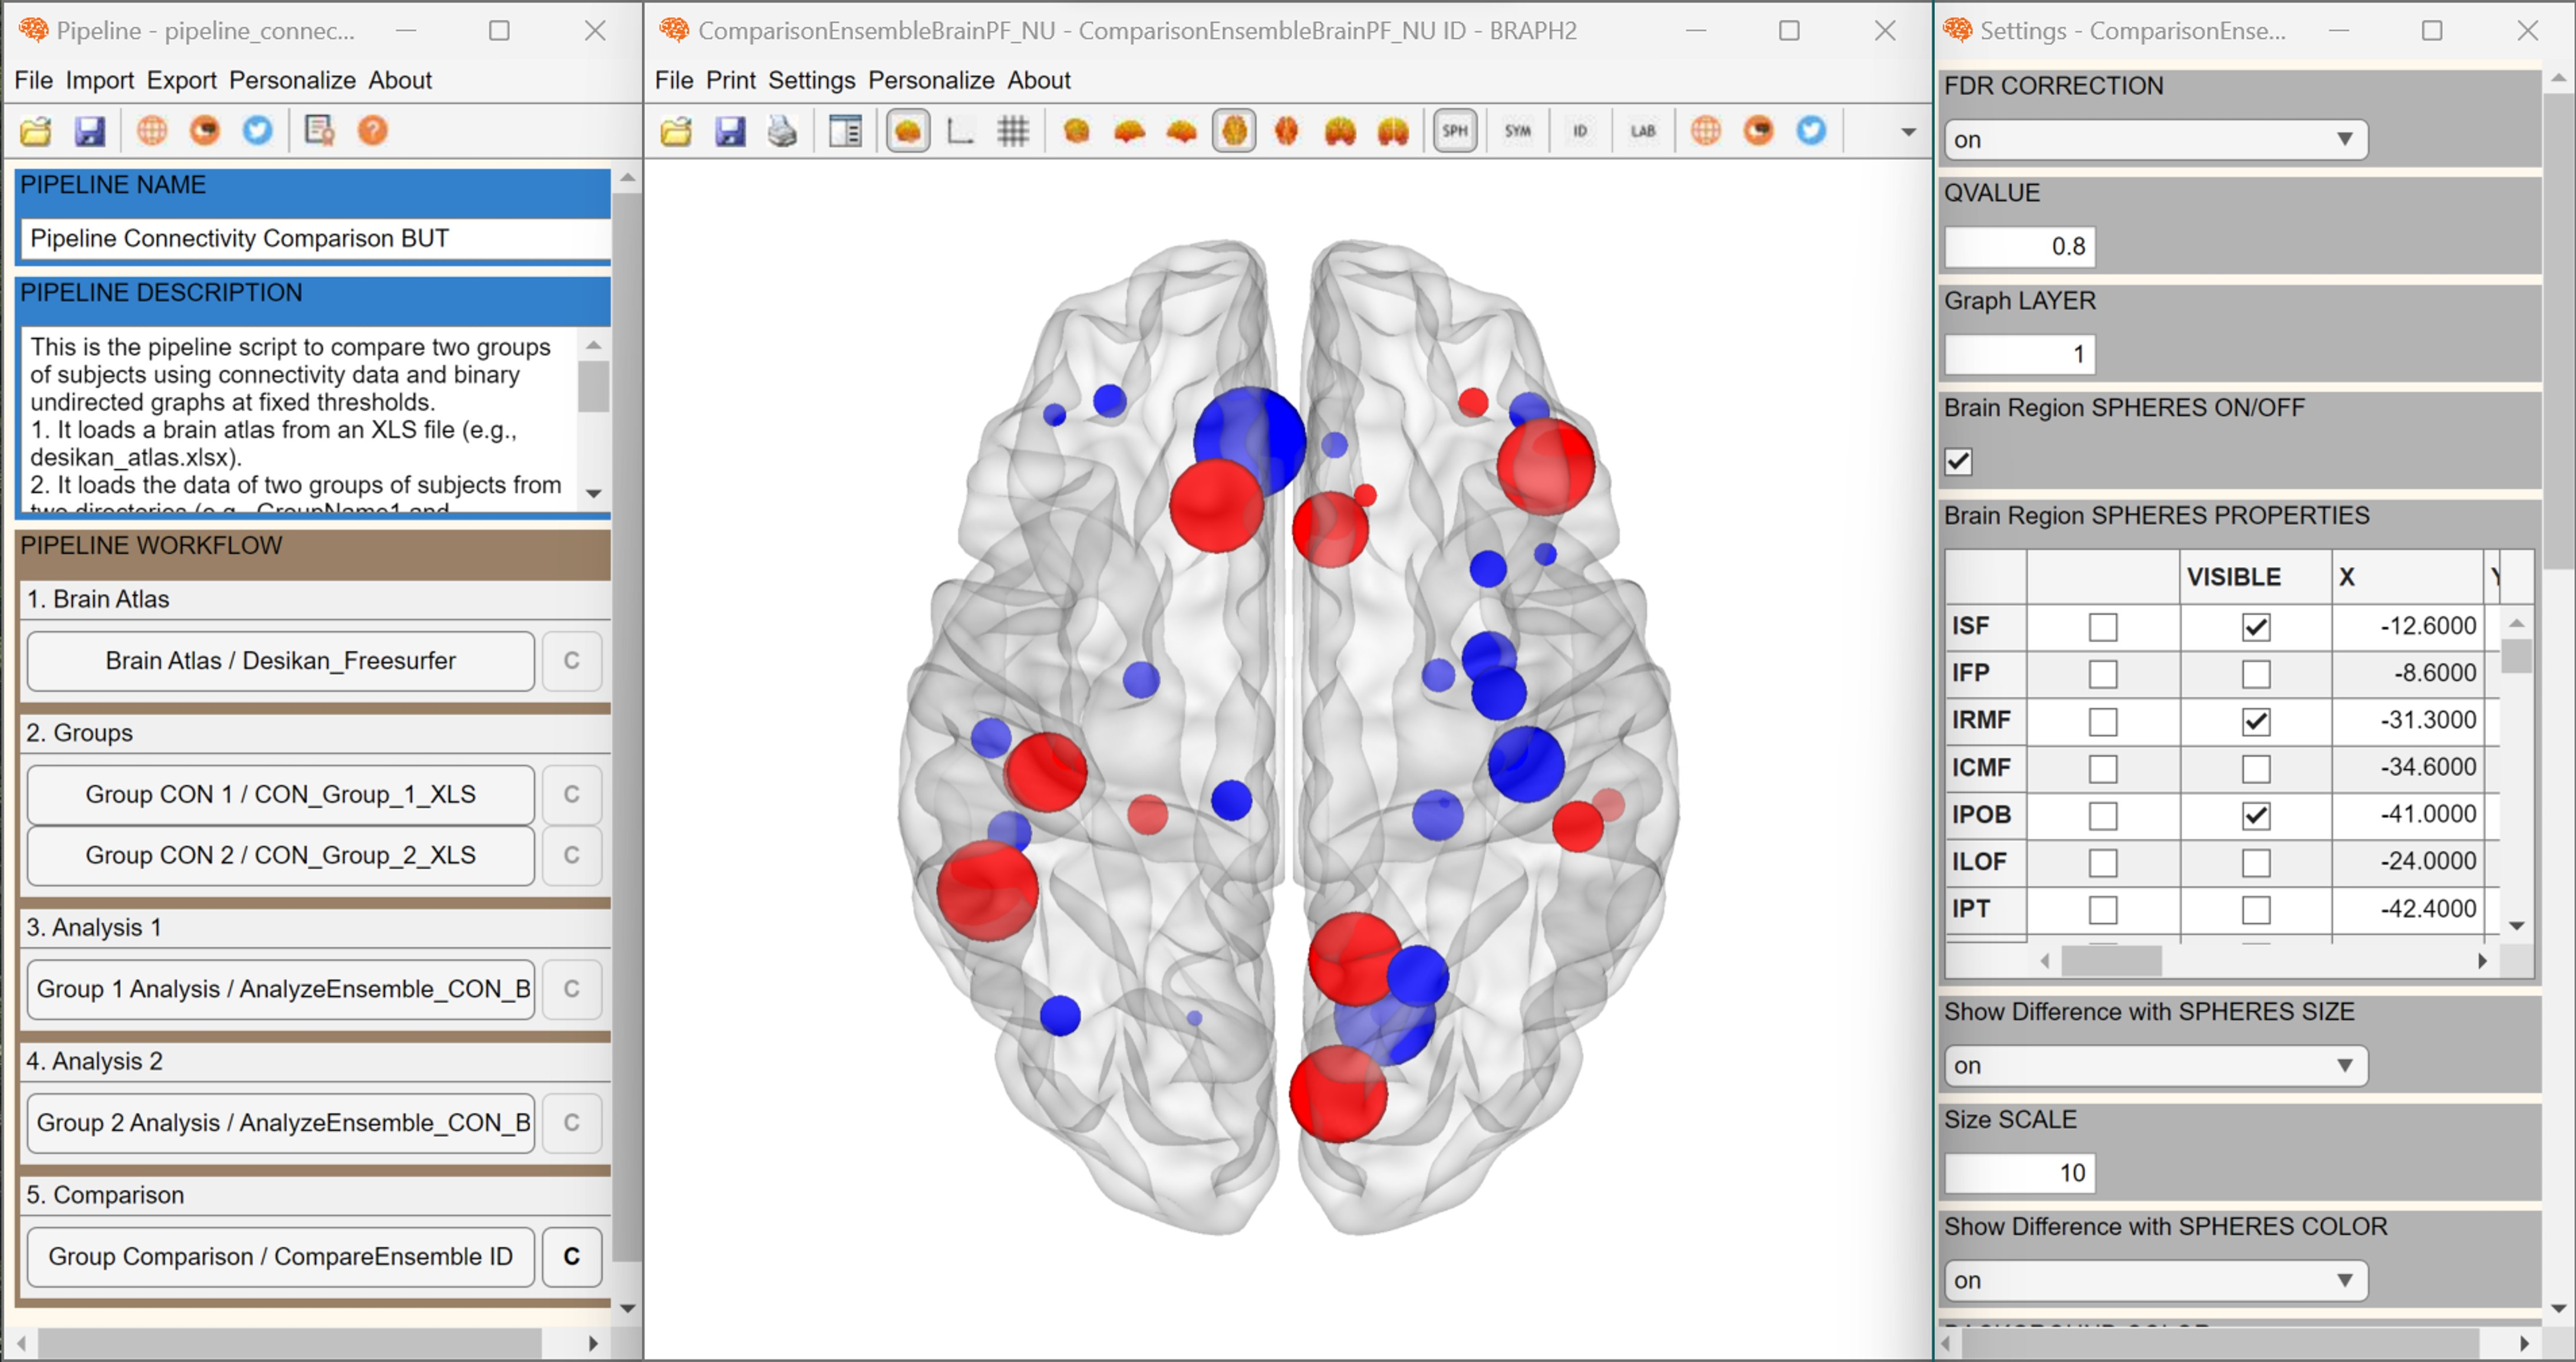
\includegraphics{fig01.jpg}}
	{GUI for working with the pipeline to compare two groups of subjects with \emph{connectivity data} using \emph{connectivity data} that has been binarised after applying different thresholds}
	{
	Full graphical user interface to perform group comparisons with \emph{connectivity data} in BRAPH~2.0. 
	}

\clearpage
\section{Generate Example Data}

You can generate the example data by typing in the command line the instruction in \Coderef{cd:generate}.
%
\begin{lstlisting}[
	label=cd:generate,
	caption={
		{\bf Command to generate example data.}
		Command to generate the example data for connectivity analyses. They will be placed in the folder \fn{./braph2/pipelines/connectivity/Example data CON XLS}, and include the brain atlas \fn{atlas.xlsx}, two folders with the subject files \fn{CON\_Group\_1\_XLS} and \fn{CON\_Group\_2\_XLS}, and the associated covariates files \fn{CON\_Group\_1\_XLS.vois} and \fn{CON\_Group\_2\_XLS.vois}. The details about the format of these files can be found in the tutorials \href{https://github.com/softmatterlab/BRAPH-2-Matlab/tree/develop/tutorials/general/tut_ba}{Brain Atlas} and \href{https://github.com/softmatterlab/BRAPH-2-Matlab/tree/develop/tutorials/general/tut_gr_con}{Group of Subjects with Connectivity Data}.
	}
]
test_ImporterGroupSubjectCON_XLS
\end{lstlisting}

\section{Open the GUI}

The general GUI of BRAPH 2.0 can be opened by typing \code{braph2} in MatLab's terminal, which allows you to select a pipeline, in this case, \emph{Pipeline Connectivity Comparison BUT}.

\fig{figure*}
	{fig:03}
	{
	%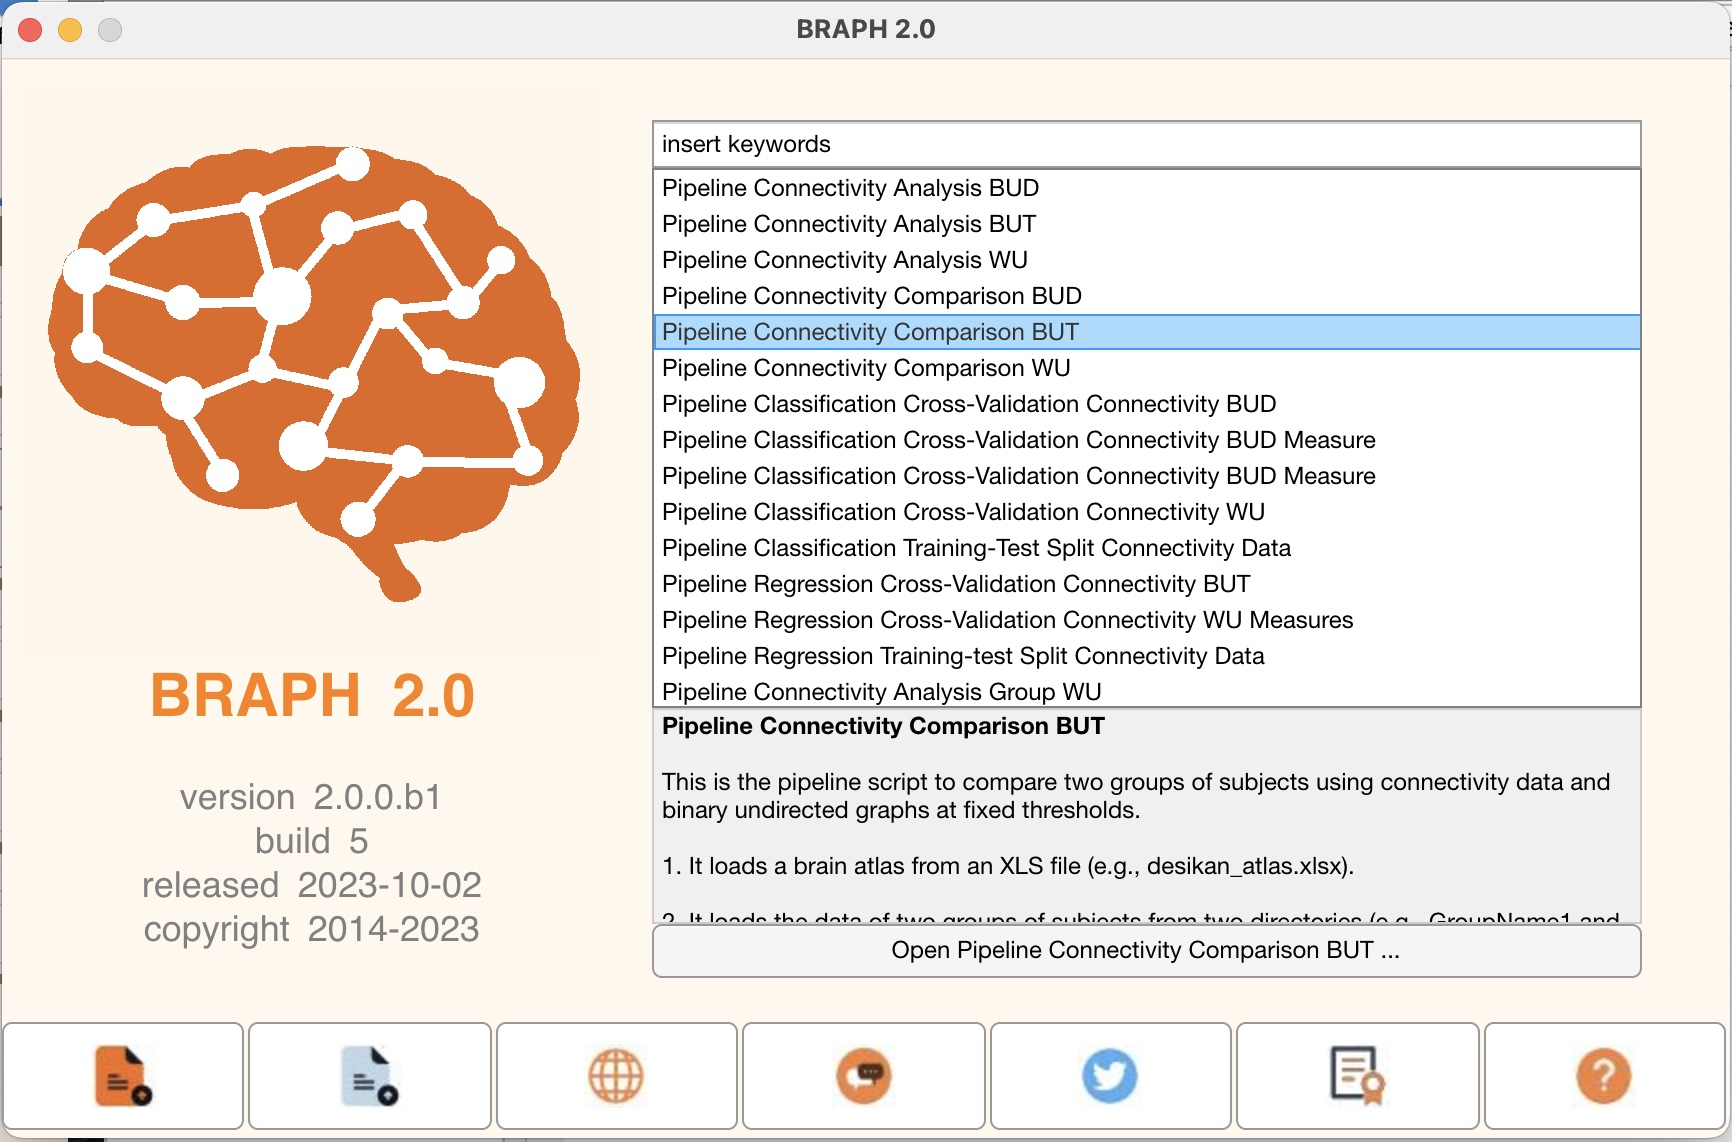
\includegraphics{fig02.jpg}
	}
	{BRAPH 2 main GUI}
	{
	BRAPH 2 main GUI with the pipeline \emph{Pipeline Connectivity Comparison BUT} selected.
	}

\begin{tcolorbox}[
	title=Pipeline launch from command line
]
To open the GUI and upload the connectivity comparison pipeline, you can also do it from the command line by typing the commands in \Coderef{cd:launch}.
%
\begin{lstlisting}[
	label=cd:launch,
	caption={
		{\bf Code to launch the GUI to upload a pipeline file to compare two groups of subjects.}
		This code can be used in the MatLab command line to launch the GUI to upload a pipeline file.
	}
]
im = ImporterPipelineBRAPH2( ...
	'FILE', which('pipeline_connectivity_comparison_but.braph2') ...
	);
pip = im.get('PIP');

gui = GUIElement('PE', pip, 'WAITBAR', true); gui.get('DRAW')
gui.get('SHOW')
\end{lstlisting}
\end{tcolorbox}

Once the pipeline is uploaded, you can see a GUI that contains different steps to: upload a brain atlas, upload the connectivity data of two groups, analyze them, and finally, compare the groups (\Figref{fig:03}a). 

\section{Step 1: Load the Brain Atlas}

\Figref{fig:03} shows how to upload and plot the brain atlas that you used to extract the \emph{connectivity data} for your analysis. For more information on where to find different atlases or how to change plotting settings on the brain surface, check the tutorial \href{https://github.com/softmatterlab/BRAPH-2-Matlab/tree/develop/tutorials/general/tut_ba}{Brain Atlas}.

\fig{figure*}
	{fig:03}
	{
	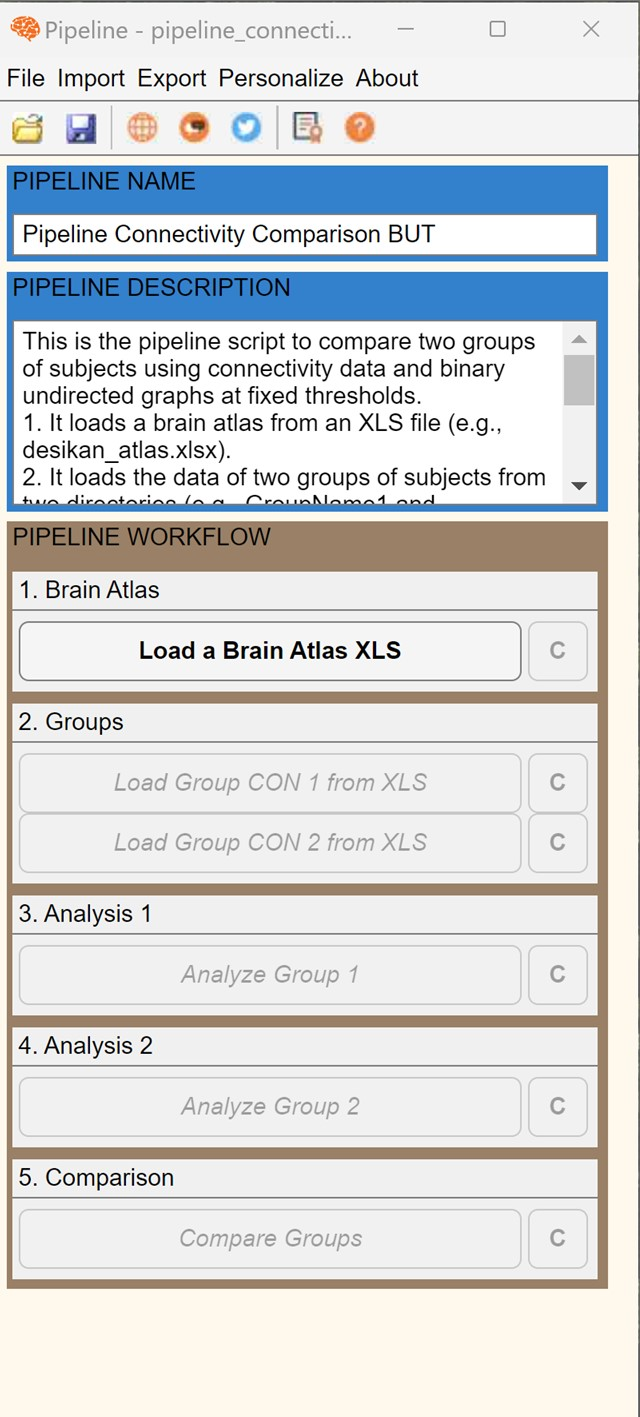
\includegraphics{fig03.jpg}
	}
	{Uploading the Brain Atlas}
	{
	Steps to upload the brain atlas:
	{\bf a} Click on \fn{Load Atlas} from the pipeline GUI.
	{\bf b} Navigate to the BRAPH~2.0 folder \fn{atlases} and select one of the atlas files, in this example the \fn{desikan\_atlas.xlsx}. {\bf c} You can visualize the brain atlas by pressing \fn{Plot Brain Atlas}. 
	}
 
\section{Step 2: Load the Connectivity Group Data}

After you loaded the brain atlas, you can upload the \emph{connectivity data} for each group as shown in \Figref{fig:04}. A new interface will be shown containing the data for the group you just selected. You can open each subject’s connectivity matrices by selecting the subject, right click, and select “Open selection” (for more information check the tutorial \href{https://github.com/softmatterlab/BRAPH-2-Matlab/tree/develop/tutorials/general/tut_gr_con}{Group of Subjects with Connectivity Data}).

%% this figure needs to be changed

\fig{figure*}
	{fig:04}
	{
	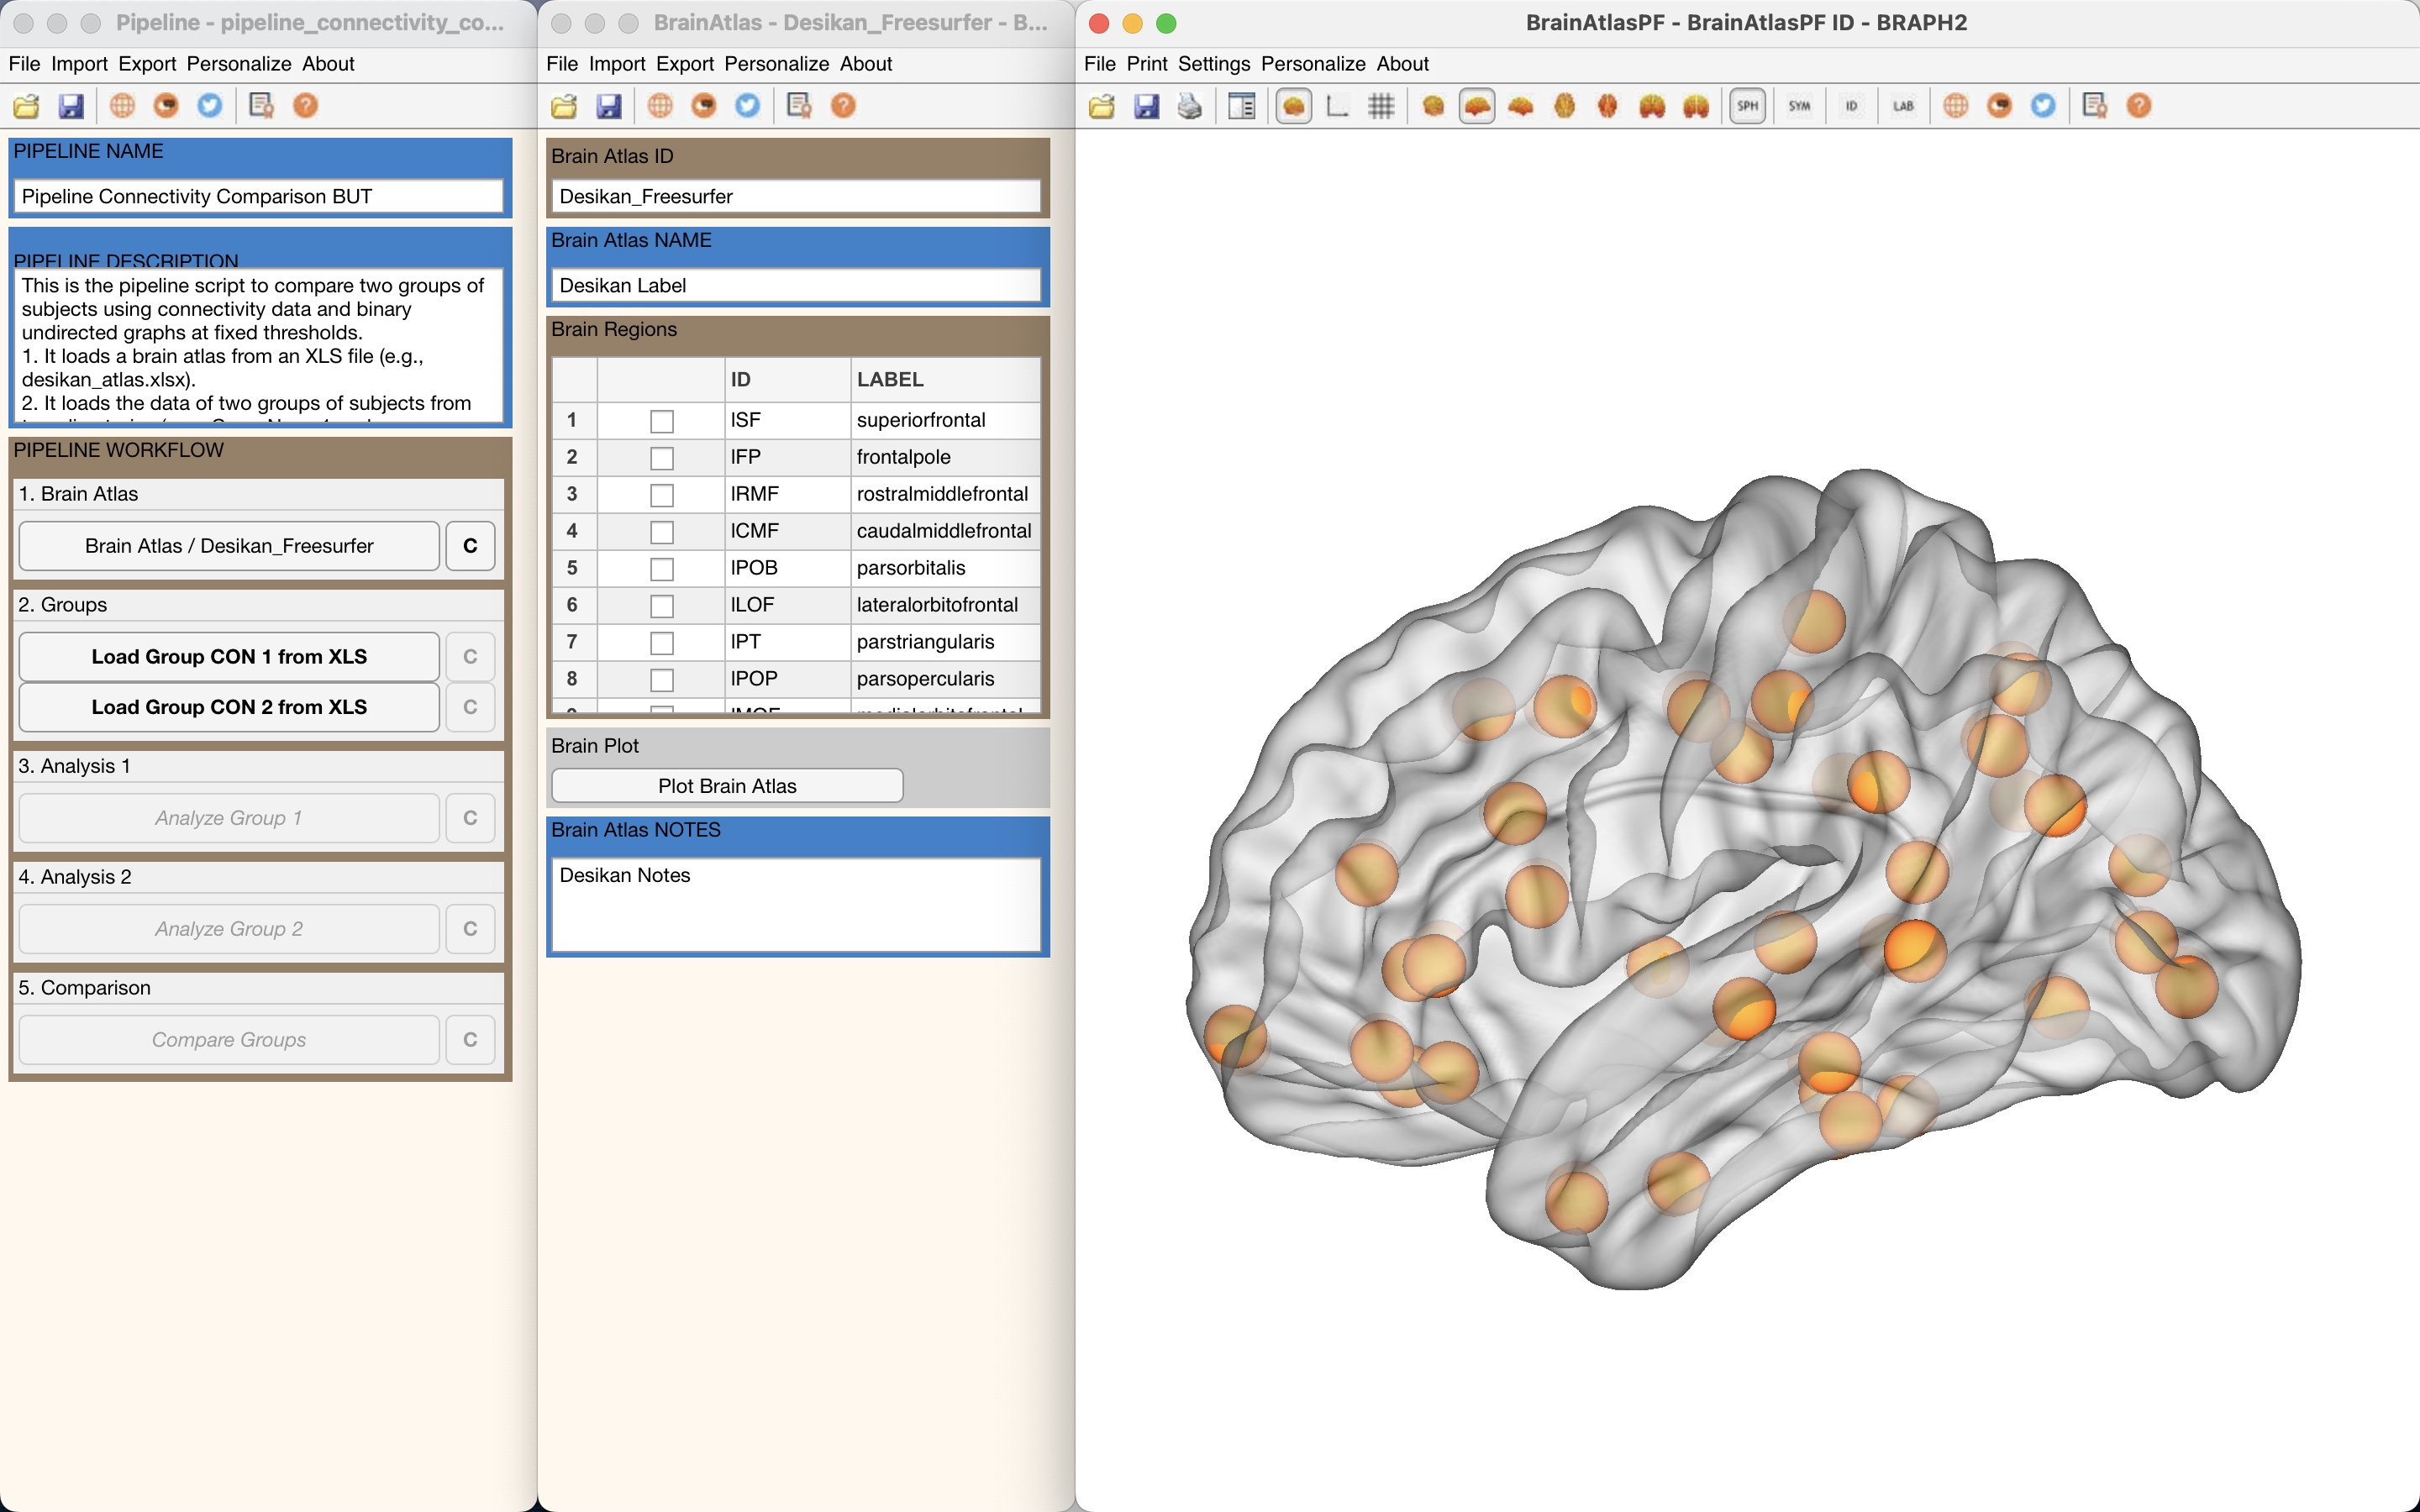
\includegraphics{fig04.jpg}
	}
	{Loading and Visualizing the Group Data}
	{
	{\bf a} From the pipeline GUI, click on \fn{Load Group CON 1 from XLS} to load the data of group 1.
	{\bf b} Once the data is uploaded, you can select a subject, right click and select "Open selection".
	{\bf c} This will open the connectivity matrix of the subject in addition to the age and sex of that subject.
	You can repeat the same procedure for group 2.
	}

\section{Step 3: Analyzing the Data of Group 1}

Once you have loaded the data for both groups, you can begin analyzing the data for the first group by clicking on \fn{Analyze Group 1} (\Figref{fig:05}a). 
This will open a new interface called \fn{Analyze Ensemble}, which allows you to pre-calculate network measures for each group and explore them. 
Before these network measures are calculated, it is important to ensure two key aspects: (1) the measures are configured with the rules or parameters you desire (note that not all measures have rules or parameters), and (2) the graph is constructed based on the thresholds you want.

Importantly, the parameters you select for this analysis, including both graph and measures parameters, will remain fixed for the analysis of the second group and for group comparisons. Let us guide you through the process of preparing these parameters for both measures and graphs.

\subsection{Setting Analysis Parameters}

In the \fn{Analyze Ensemble} interface (\Figref{fig:05}e) you can configure the analysis parameters.
In the \fn{THRESHOLDS} section, you can define the thresholds by entering values like ``[0.4 0.5 0.6 0.7]'' or ``0.4:0.1:0.7''. 
In this tutorial, we will stick with the default thresholds. 

\subsection{Setting Parameters for Graphs}

To configure the measure parameters, start by clicking on \fn{Graph Template} (\Figref{fig:05}b). This will open a new interface for graph template settings. 
In brain connectivity analysis, threshold values dictate the required connection strength between different brain regions for them to be considered “connected” in a binary undirected graph. 
Adjusting these thresholds allows you to explore varying levels of brain connectivity, providing insights into how regions communicate at different threshold settings.

\subsection{Setting Rules for Measures}

Scroll down to find the \fn{Graph MEASURES} section. 
By clicking the 'C' button, all compatible measures will be displayed in a table. 
For example, you can select the \fn{Community Structure} measure and then right-click at the top of the table (\Figref{fig:05}c). 
In the right-click menu, choose “Data Selected Measures.” 
This will open the measure window, allowing you to specify the rules or parameters (\Figref{fig:05}d).

\fig{figure*}
	{fig:05}
	{
	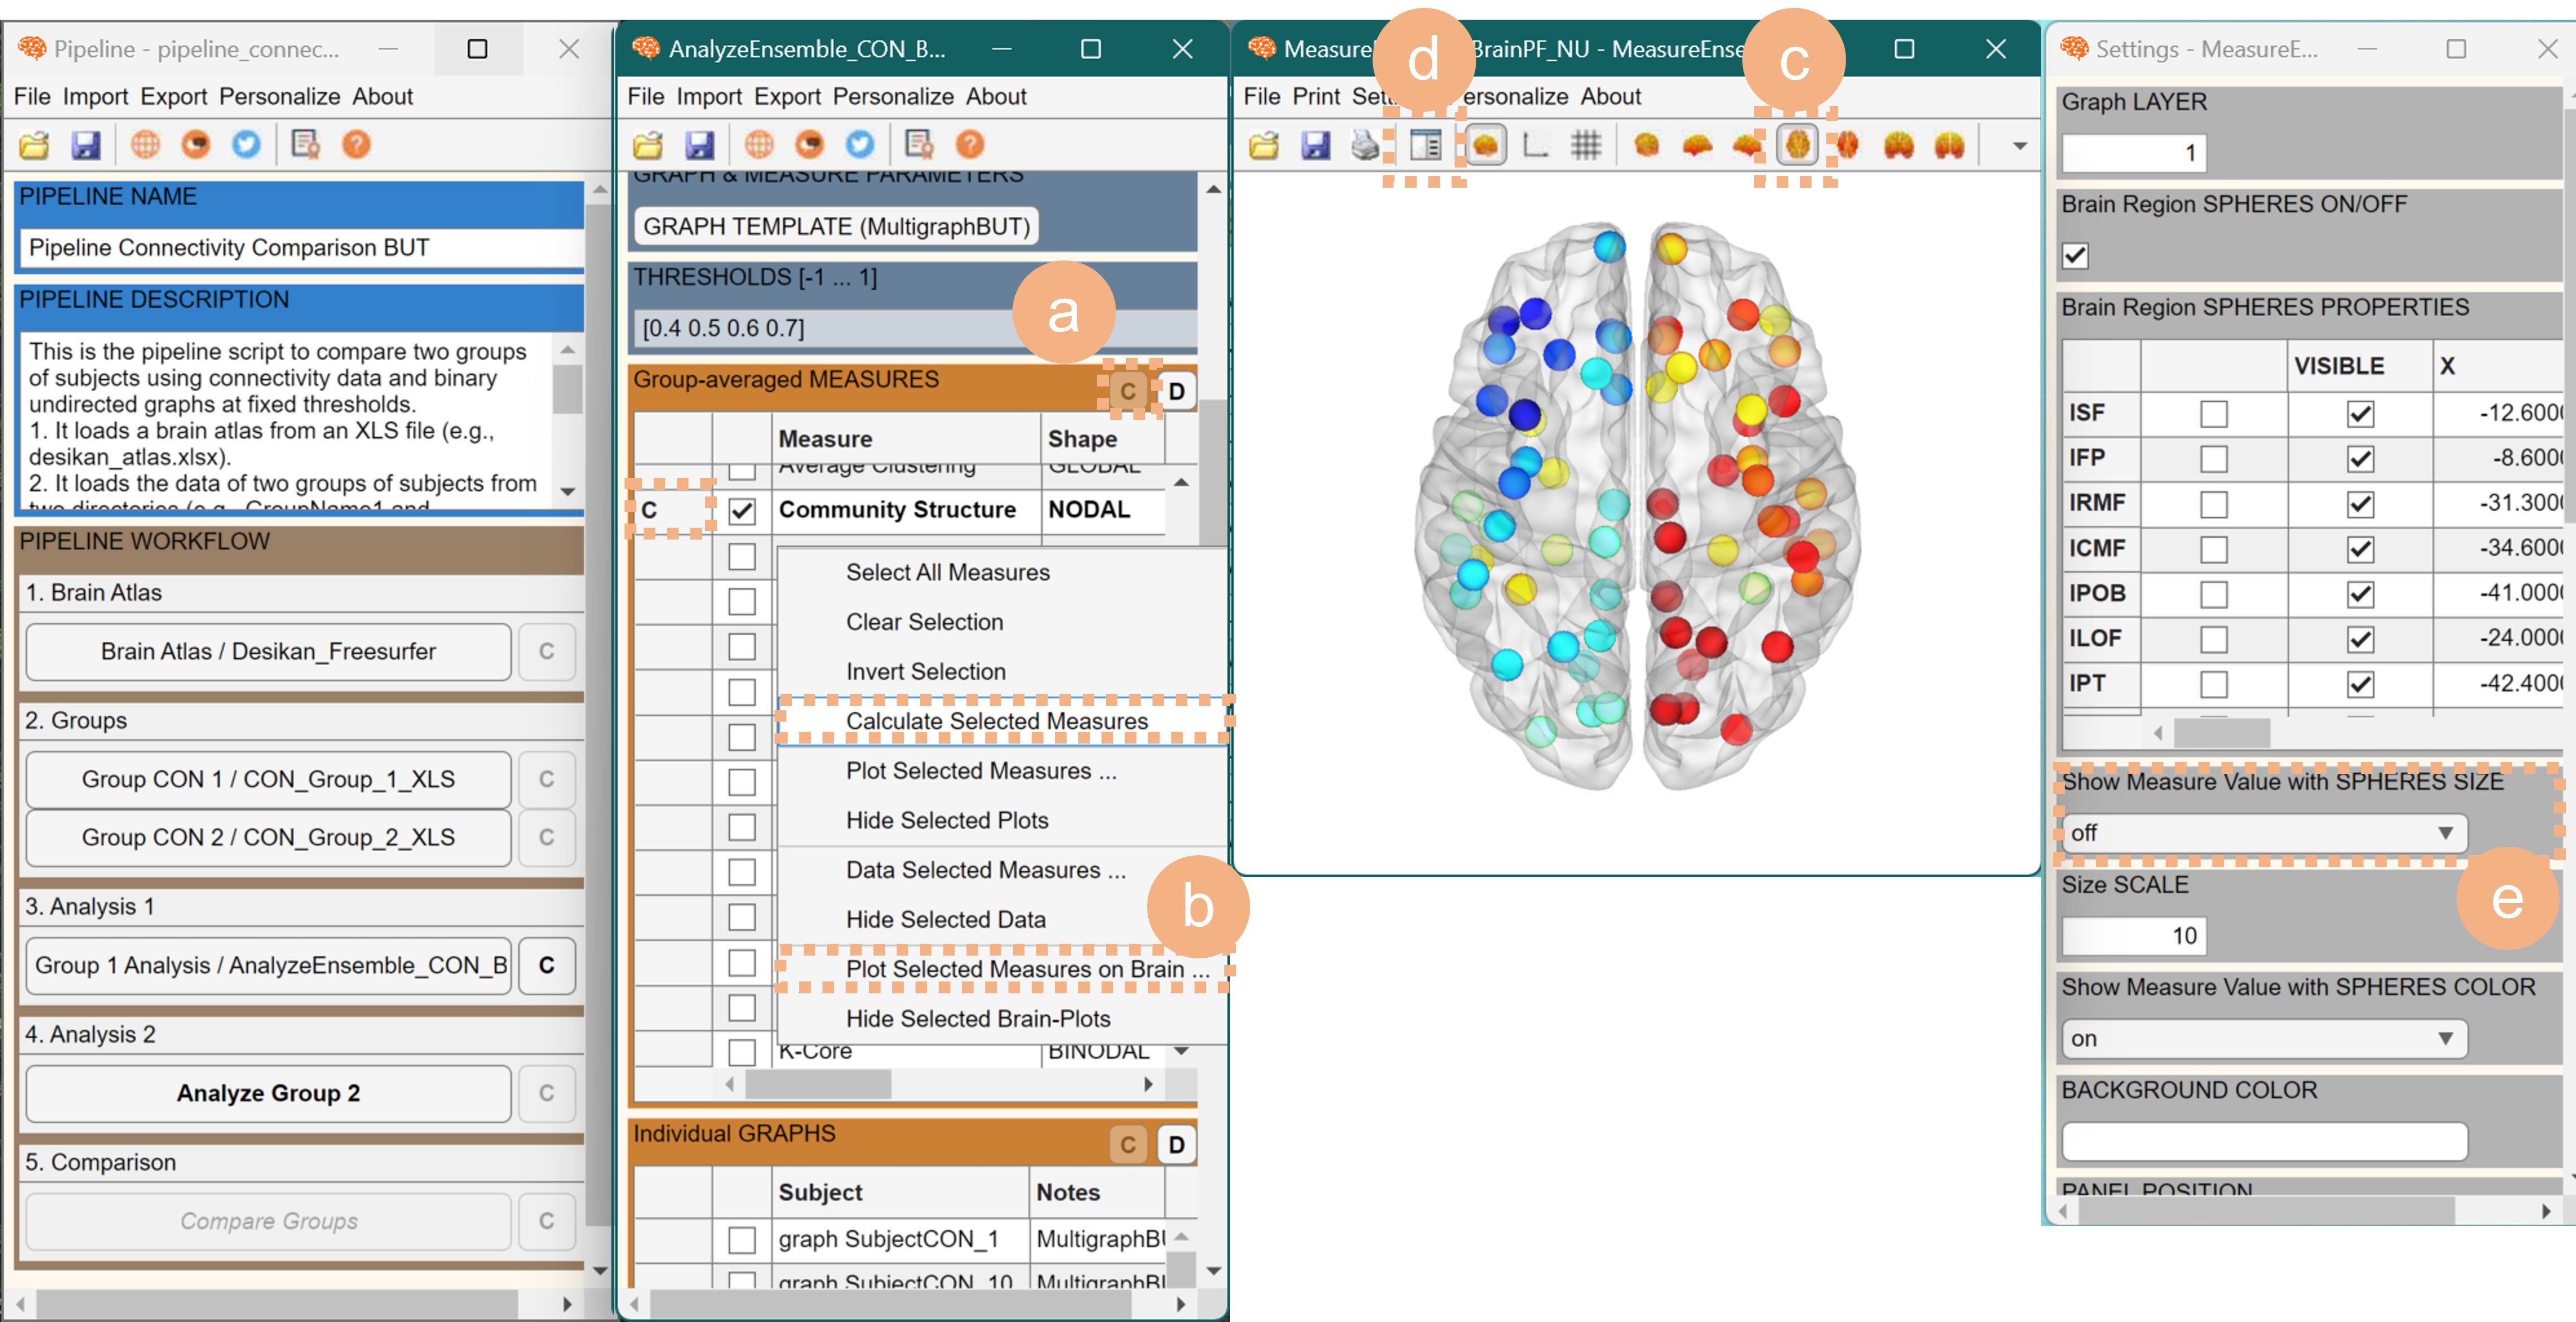
\includegraphics{fig05.jpg}
	}
	{Configuring Measure Rules and Parameters Before Calculation}
	{
	{\bf a} To initiate the analysis of data for group 1, click on \fn{Analyze Group 1}.
	{\bf b} Access the graph template settings by clicking on \fn{GRAPH TEMPLATE}, opening a new interface.
	{\bf c} Inside this interface, you'll find the \fn{Graph MEASURES} panel. Click the 'C' button to reveal a table displaying all compatible measures. Select the \fn{Community Structure} measure and then right-click at the top of the table. In the right-click menu, choose “Data Selected Measures.”
	{\bf d} The measure window that opens allows you to define the rules or parameters for the \fn{Community Structure} measure.
	{\bf e} After configuring the measure rules, return to the \fn{Analyze Ensemble} interface to set the thresholds.
	}

\fig{figure*}
	{fig:06}
	{
	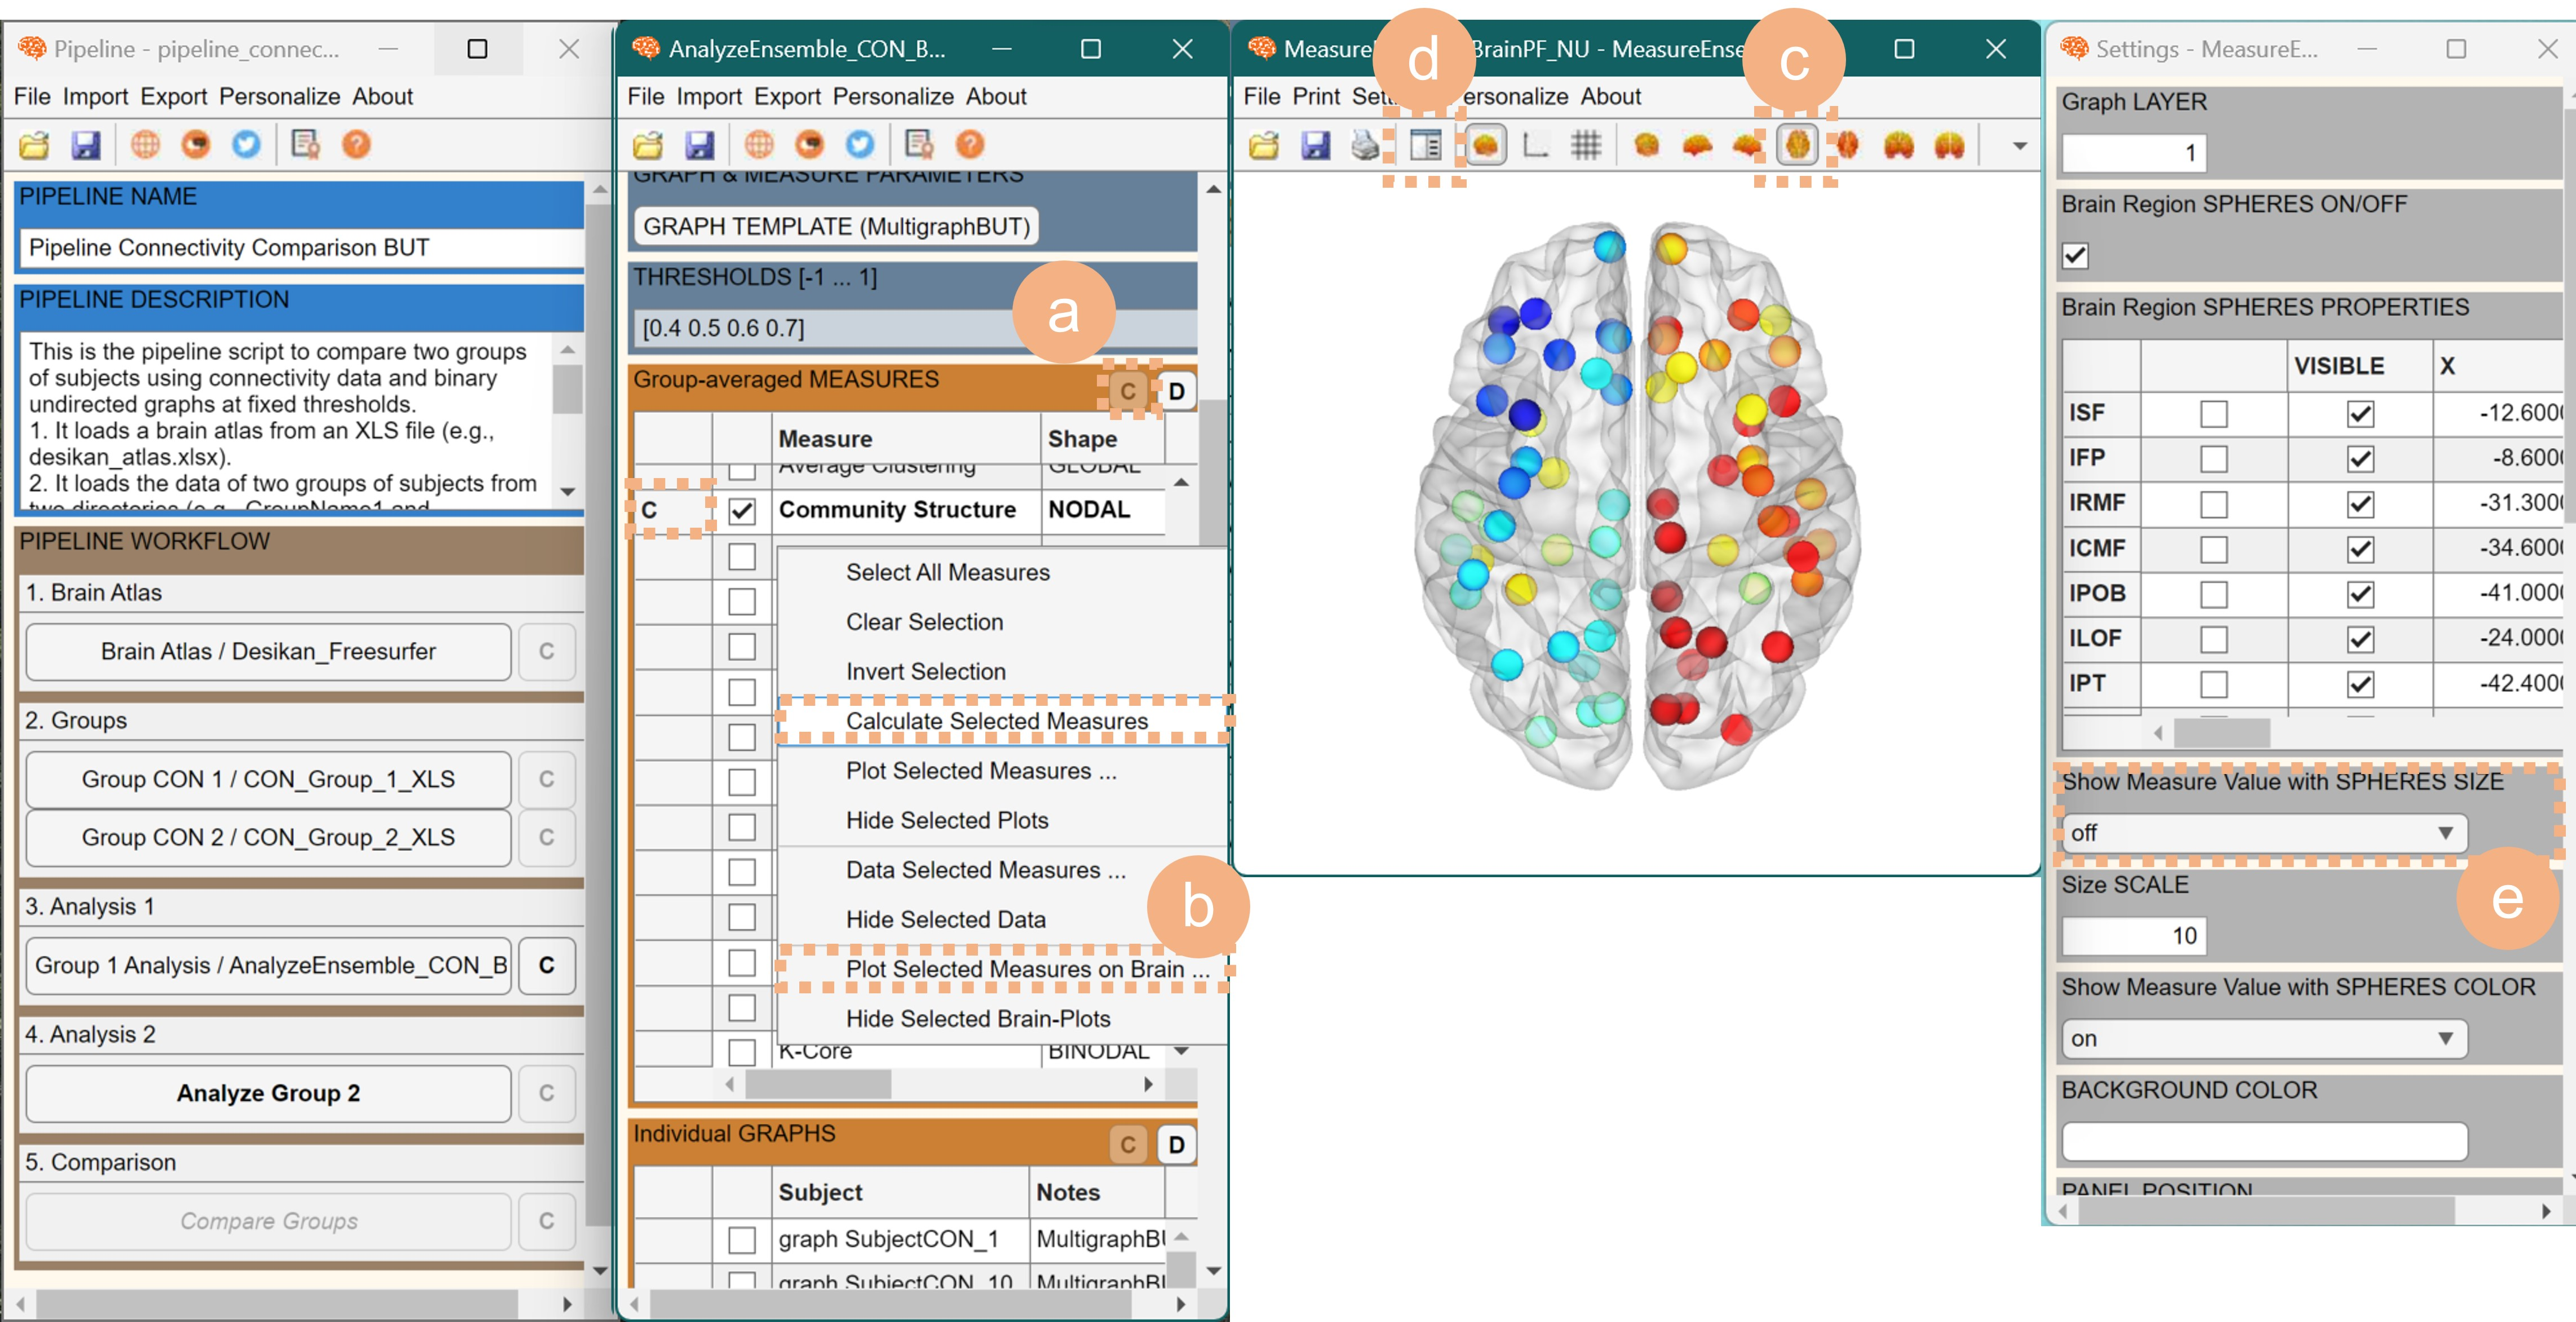
\includegraphics{fig06.jpg}
	}
	{Analyzing the Group Data}
	{
	{\bf a} Locate the \fn{Group-averaged MEASURES} panel and click the 'C' button to see all available measures. Choose the \fn{Community Structure} measure, right-click it, and select “Calculate Selected Measures” to perform the calculation.
	{\bf b} To visualize the results, right-click on the top of the table and choose \fn{Plot Selected Measures on Brain} in the Analyze Ensemble interface. This action opens a brain surface with the \fn{Community Structure} plotted.
	{\bf c} Explore different views such as the “Axial dorsal” button in the brain surface toolbar.
	{\bf d} Adjust visualization settings by clicking on the “Settings Panel Figure” button in the same toolbar.
	{\bf e} Customize and save plot visualizations within the settings menu. Here, we turned off the option to show the spheres corresponding to the nodes of each community with different sizes.
	}
 
\subsection{Calculate Measures}
 
After configuring these parameters, you can proceed to calculate specific graph measures (\Figref{fig:06}). To do this, return to the \fn{Analyze Ensemble} interface (\Figref{fig:06}a) and scroll down to locate the \fn{Group-averaged MEASURES} panel. By clicking the 'C' button, you will see a table displaying all measures.

As an illustrative example, let us select the \fn{Community Structure} measure, for which we previously set the rule to \fn{louvain}. Right-click at the top of the table and choose “Calculate Selected Measures.” Once the calculation is complete, you will notice a \fn{C} appearing in front of the \fn{Community Structure}, indicating that this measure has been calculated.

If you wish to visualize the results, right-click on the top of the table and select \fn{Plot Selected Measures on Brain} within the Analyze Ensemble interface (\Figref{fig:06}b). This will open a brain surface with the \fn{Community Structure} plotted on it.

Within the toolbar of the brain surface interface, you can explore various views.
For instance, by clicking on the “Axial dorsal” button (\Figref{fig:06}c), you will get the same view as shown in \Figref{fig:06}. Additionally, clicking on the “Settings Panel Figure” button (\Figref{fig:06}d) in the same toolbar allows you to adjust different visualization settings.

For instance, within the settings menu (\Figref{fig:06}e), you can disable the size effect, resulting in the same kind of figure as shown in \Figref{fig:06}d. Within the settings menu, you can customize the visualization of the plots and save them for reference.

Finally, when you right-click in the \fn{Group-averaged MEASURES} panel, you will find other options to explore, such as \fn{Plot Selected Measures} (which generates a line plot for the selected measure at different thresholds and/or different nodes) and \fn{Data Selected Measure} (providing the calculated values of the selected measures). These options can also be saved for further analyses outside BRAPH 2.0.

\section{Step 4: Analyzing the Data of Group 2}

After completing the analysis of Group 1, you can analyze the second group by simply clicking on \fn{Analyze Group 2} (\Figref{fig:07}a). You will notice that in the new GUI (\Figref{fig:07}b-d), the parameters you previously selected for Group 1 for graph and measure settings are already preselected and fixed for this analysis. 

If you want to change some of the options you previously selected for Group 1 you can reset the analysis parameters for Group 1 by clicking on the checkbox marked with a 'C' (\Figref{fig:07}e) next to the settings of Group 1.


\fig{figure*}
	{fig:07}
	{
	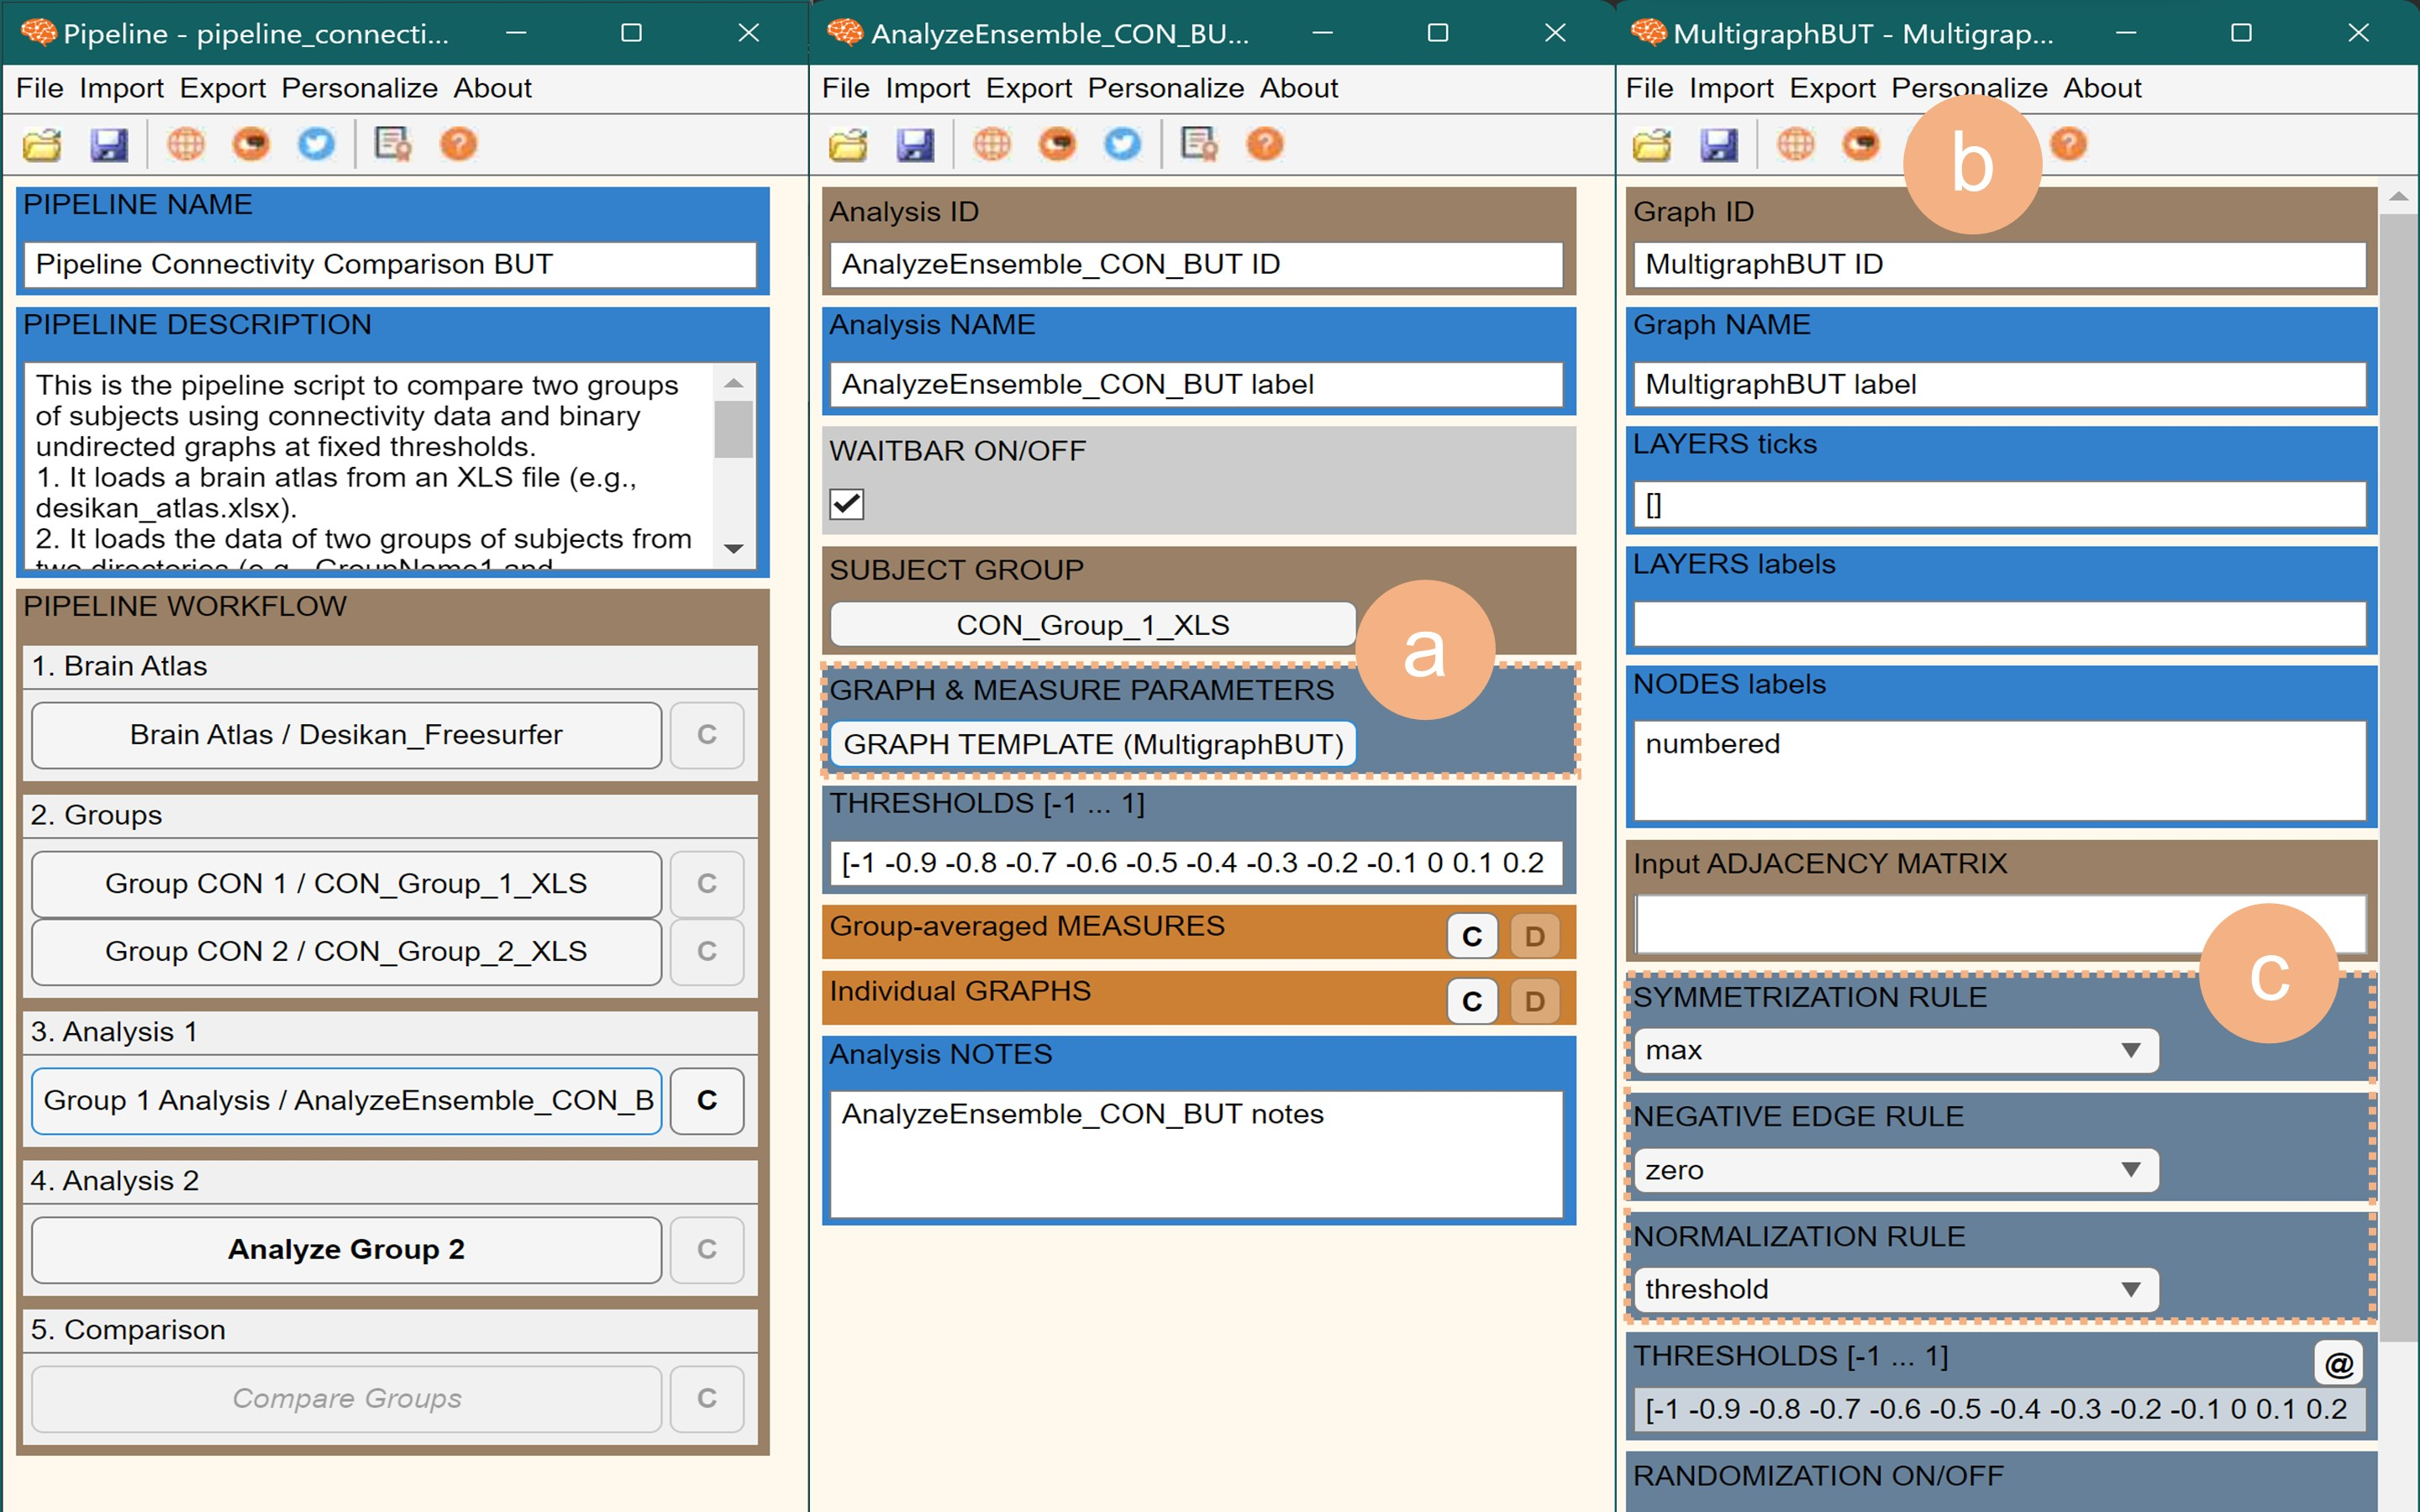
\includegraphics{fig07.jpg}
	}
	{Parameters blocked in the Analysis of Group 2}
	{
	{\bf a} Click on \fn{Analysis 2} in the pipeline's GUI.
	{\bf b} In this new window, you can see that the measure parameters, such as the {\bf b} \fn{GRAPH TEMPLATE} and {\bf c} rule for \fn{Community Structure}, as well as the graph property {\bf d} \fn{THRESHOLDS}, are blocked since they should be the same as the ones set in the analysis of group 1. You can reset the analysis parameters for Group 1 by clicking on the checkbox marked with a 'C' next to the settings of Group 1 {\bf e}.
	}
 
\section{Step 5: Comparing Groups}

After exploring the network measures for each group, you can proceed to their statistical comparison by clicking on \fn{Compare Groups} (\Figref{fig:08}a).

In the new window, you have several options to configure the analysis. First, you can choose whether to enable a progress bar and verbose functions while the analysis is running, which can help you monitor the progress of the analysis. You can also specify how many permutations you want to use to assess differences between groups (\Figref{fig:08}b).

If your groups are not independent and represent the same subjects assessed in different points in time, you can select the longitudinal comparison option. This option will permute the values within each subject, considering their temporal relationship (\Figref{fig:08}b).

For computational efficiency, in this tutorial we have set the number of permutations to 10. However, for your research analysis, we recommend using a higher number, such as 1000 or 10000 permutations, to ensure the results are robust.

Next, you can select the specific graph measures you wish to compare between the groups. To do this, click on “C” in the \fn{COMPARISONS} section (\Figref{fig:08}c). Once you have chosen all the measures of interest, right-click and select \fn{Calculate Selected Comparisons}.

If you have enabled the progress bar and verbose functions, two additional windows will appear to display the progress of the comparison calculations. Finally, there is an option in this GUI to save intermediate results during the permutations, which can be helpful for further analysis.

\fig{figure*}
	{fig:08}
	{
	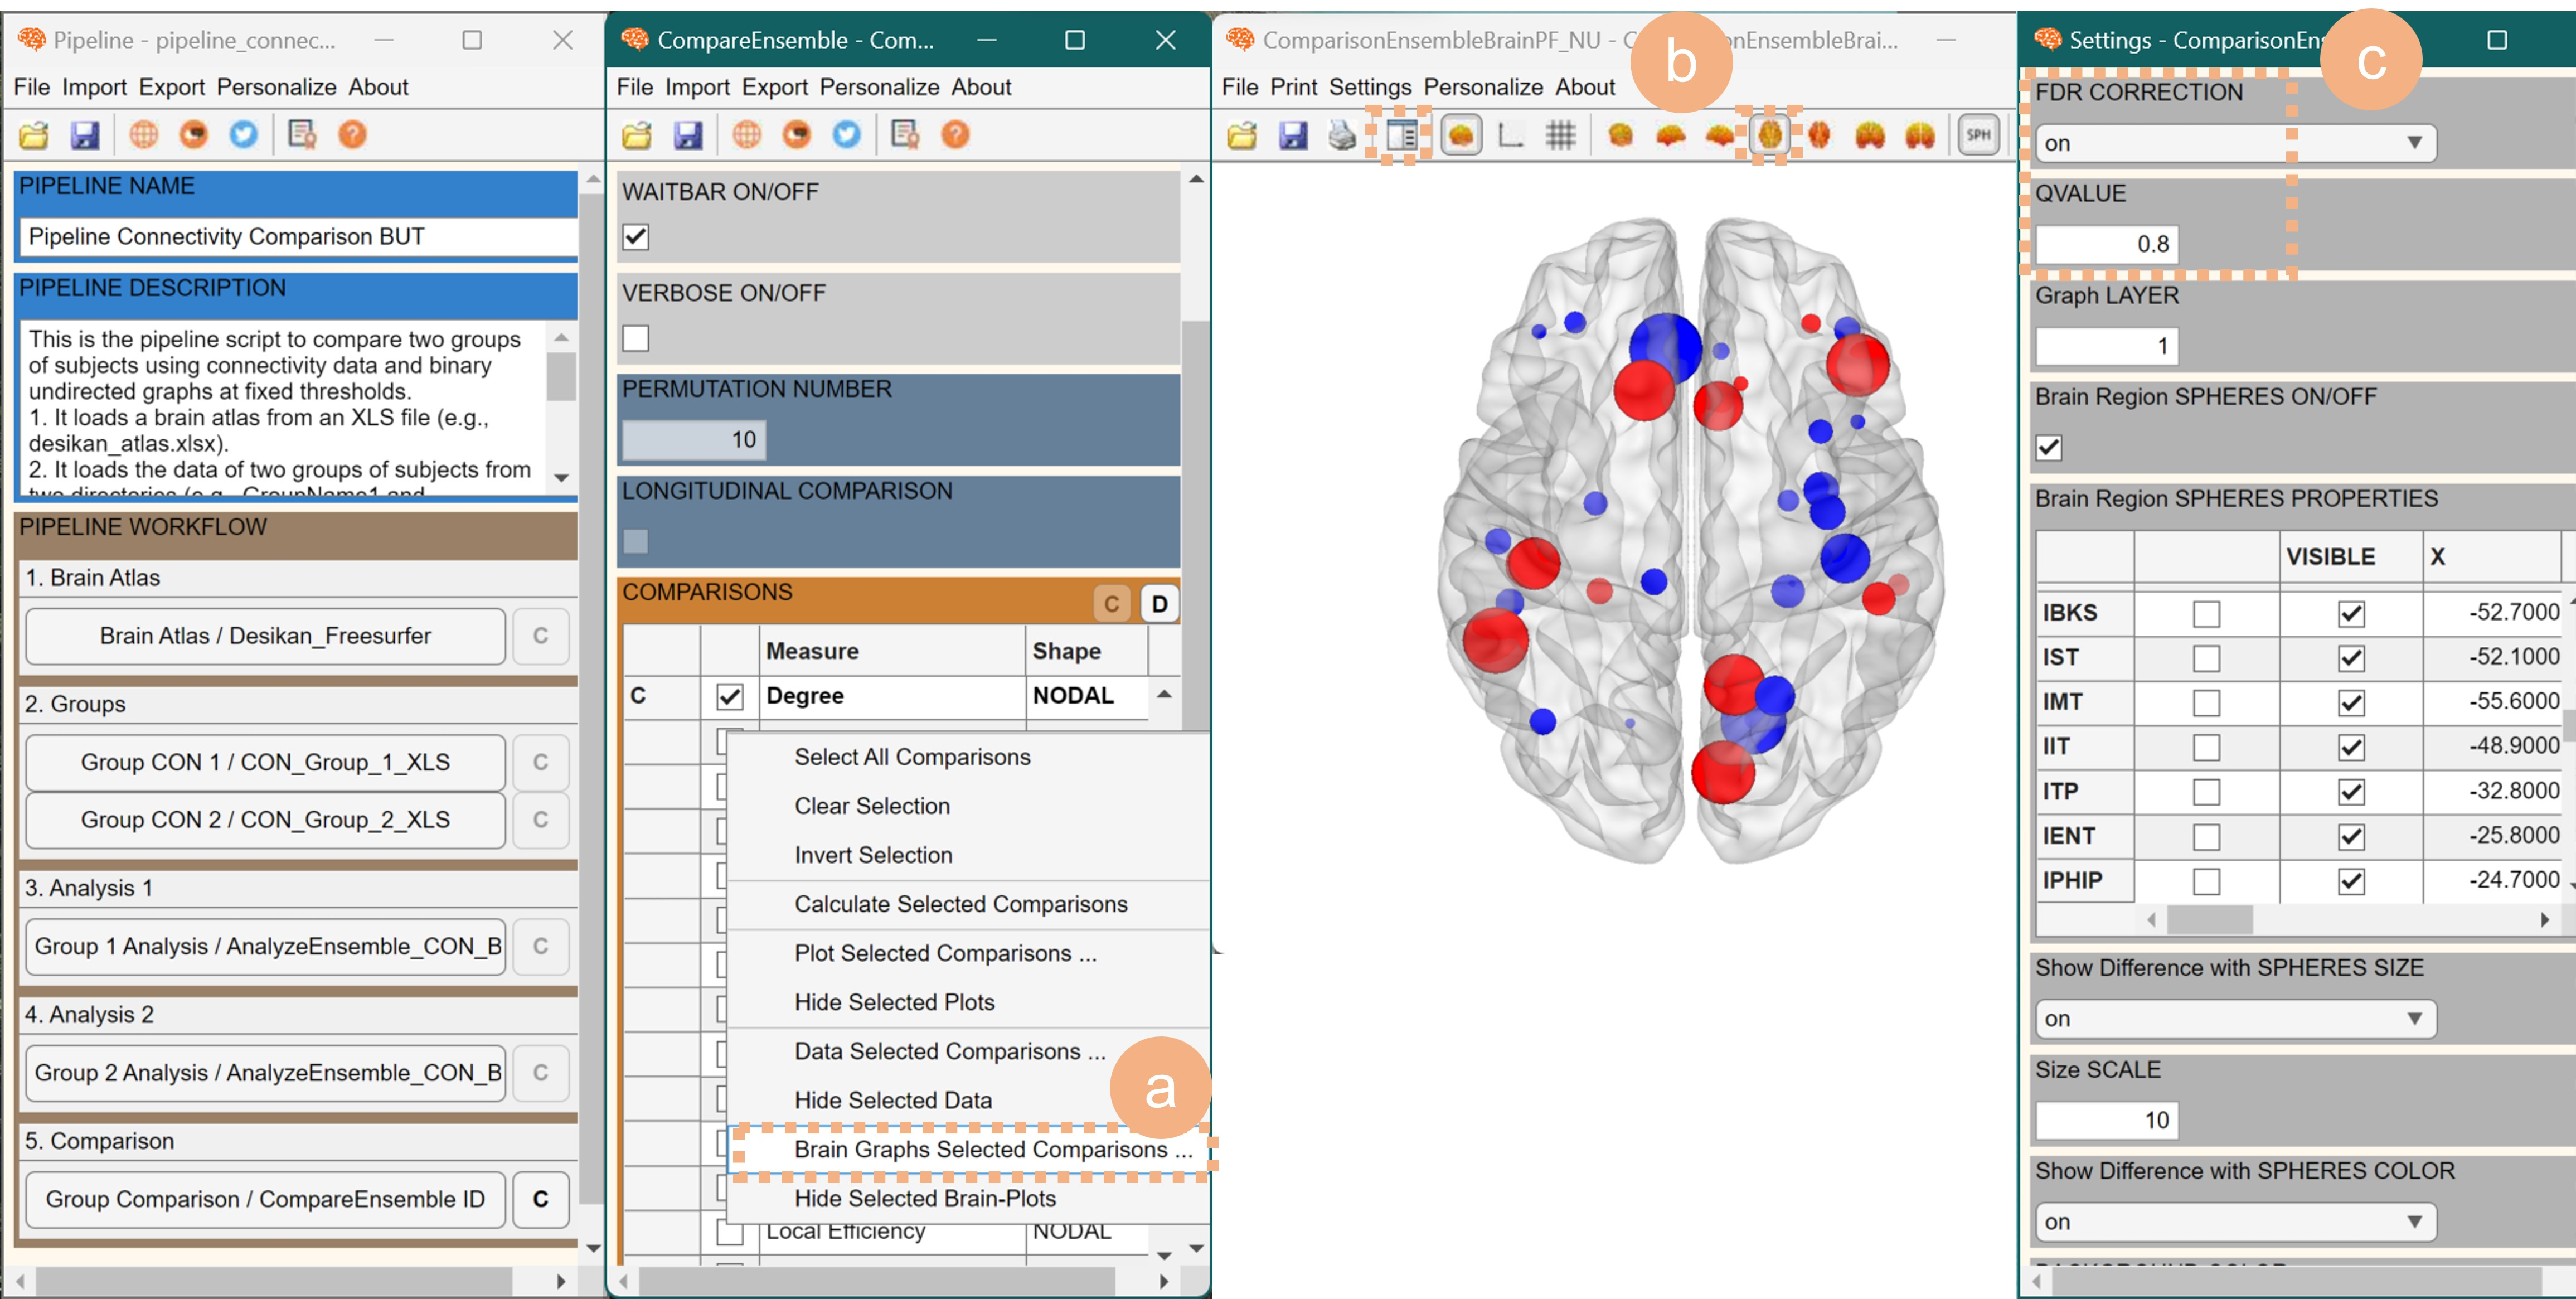
\includegraphics{fig08.jpg}
	}
	{Compare the Group Data}
	{
	{\bf a} Click on \fn{Compare Groups} in the pipeline's GUI.
	{\bf b} In this new window, you can select to turn ON/OFF the wait bar and verbose functions, you can change the number of permutations, and whether to perform a longitudinal group comparison. We set the number of permutations to 10 for this tutorial {\bf c}. Finally, you can calculate the comparisons of some graph measures between groups {\bf d}.
	}
 
To obtain the results from the comparisons, select the measures in the \fn{COMPARISONS} panel and press \fn{Data Selected Comparisons}({\Figref{fig:08}d}), and a new window will open where we can check the value of the difference between groups, the p-values (1-tailed and 2-tailed), as well as the confidence intervals.

 \fig{figure*}
	{fig:09}
	{
	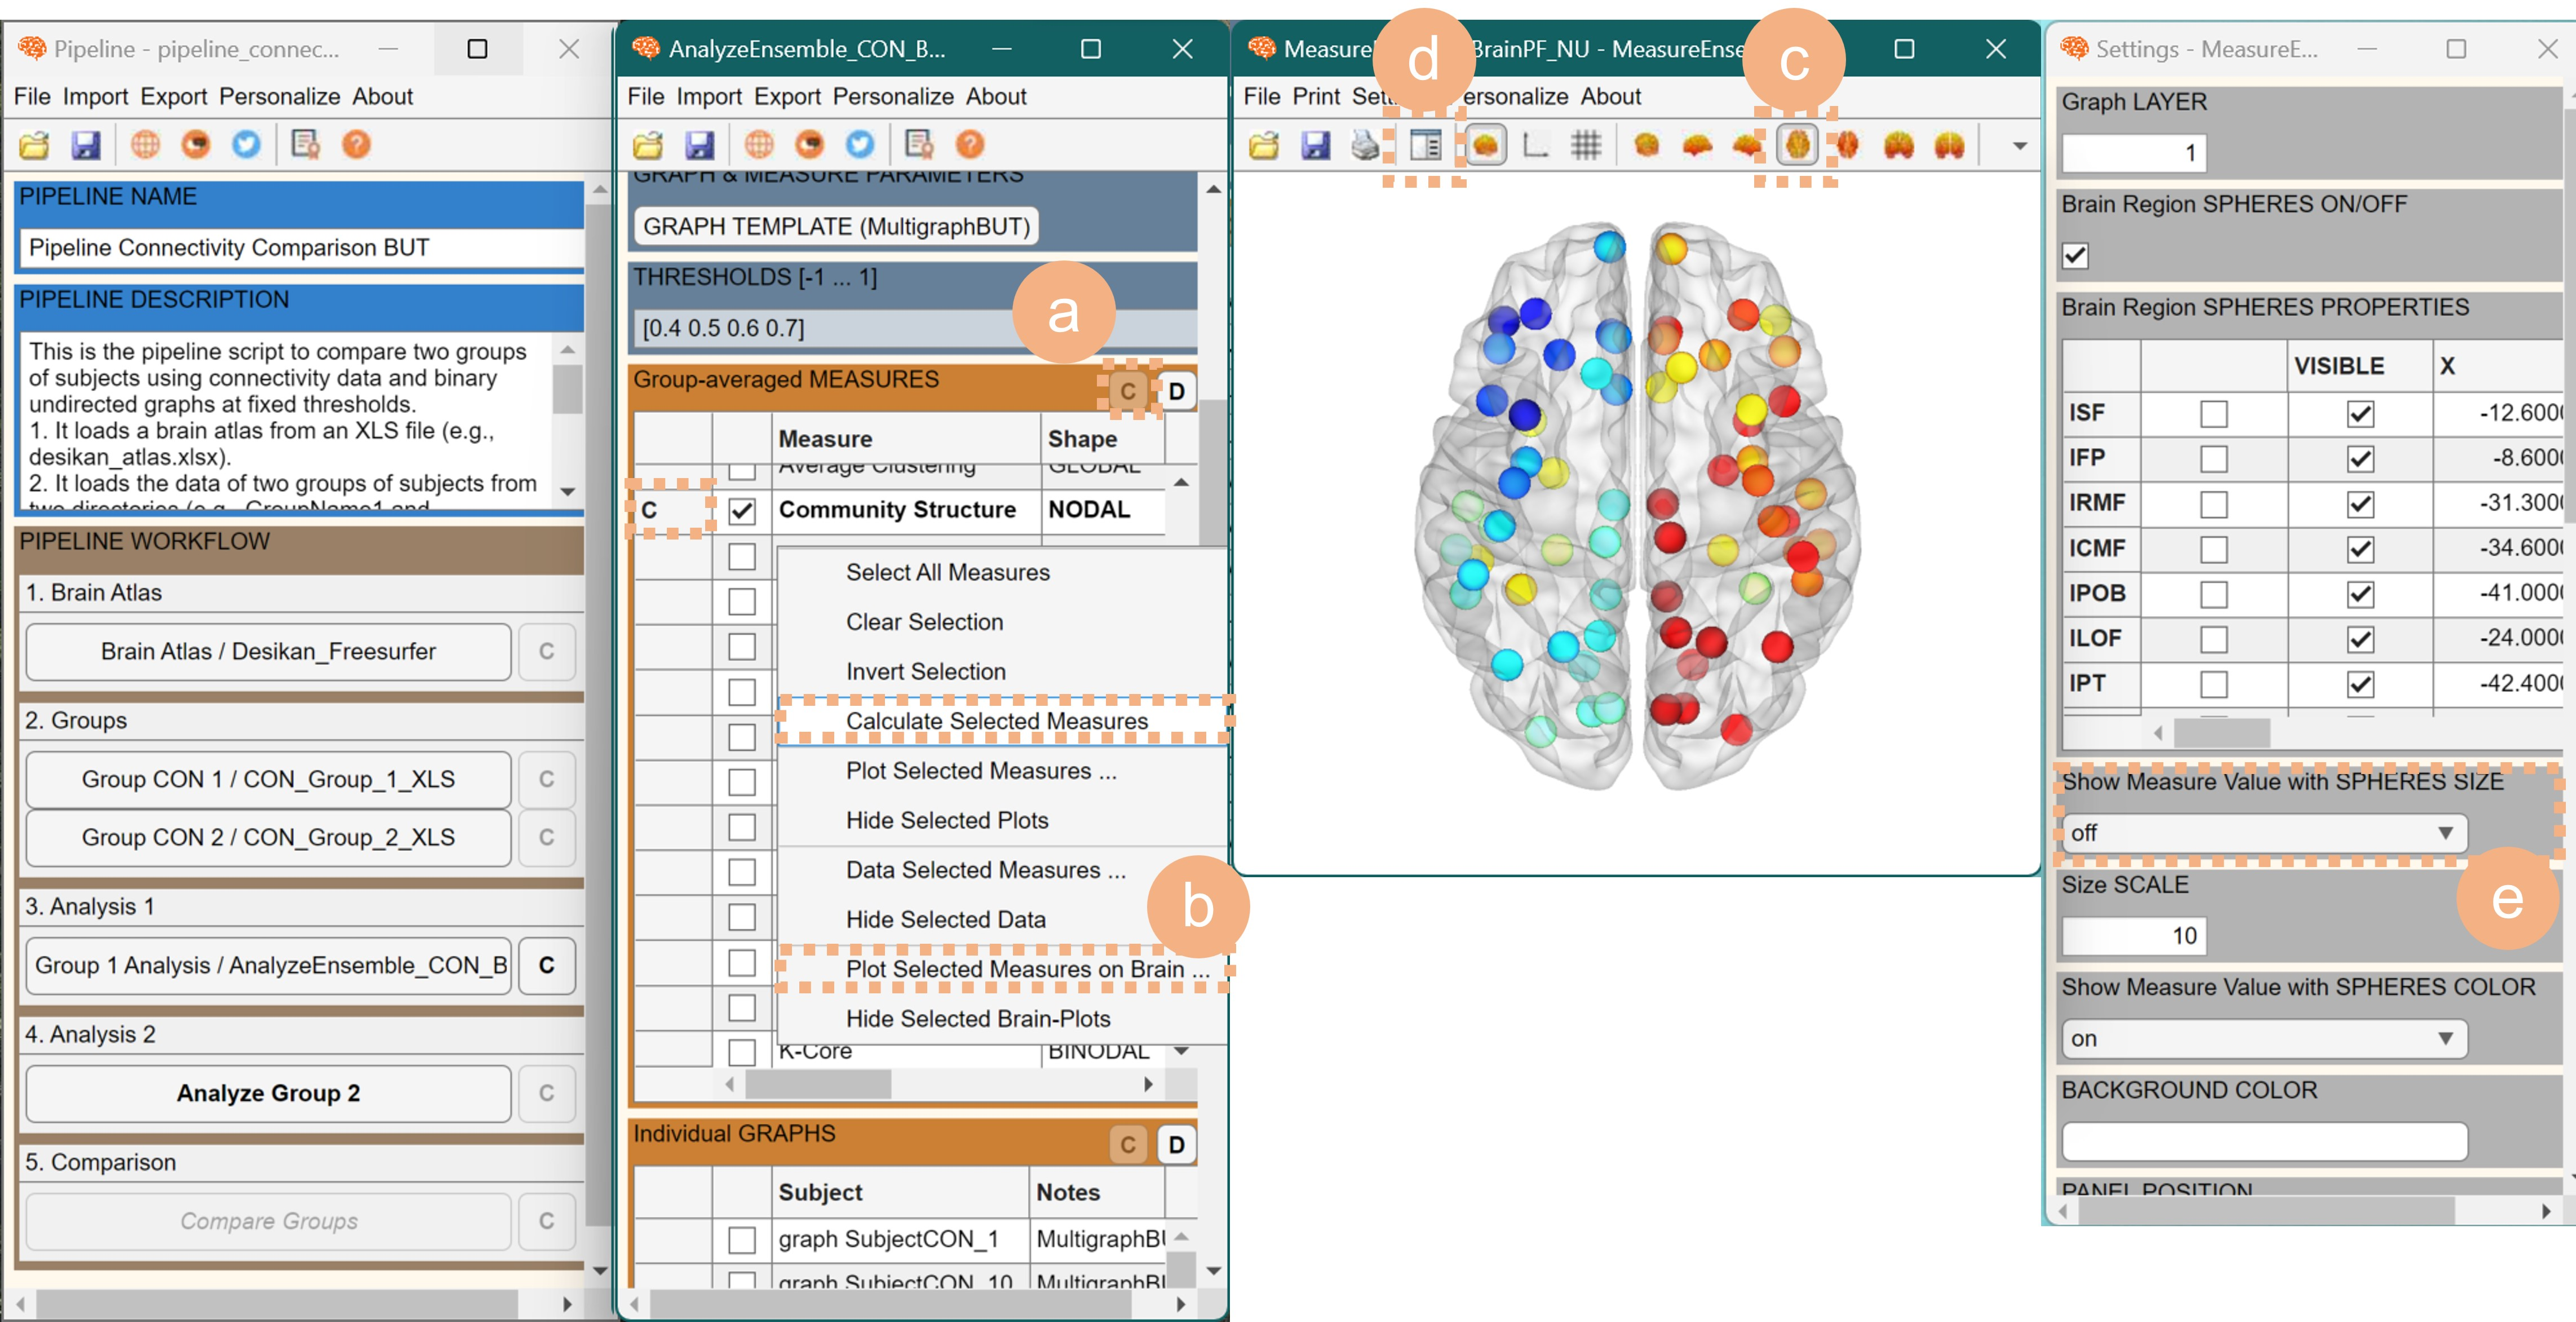
\includegraphics{fig09.jpg}
	}
	{Visualize the group comparison results on a brain surface}
	{
	{\bf a} Click on \fn{Brain Graph Selected Comparison} in the Comparisons panel.
	{\bf b} In this new window, you will see the comparison results, with positive values in red and negative values in blue on the brain surface.
{\bf c} You can customize this visualization using the settings menu.
	}

If you wish to visualize the results, right-click at the top of the table and select \fn{Brain Graph Selected Comparison} within the Compare Ensemble interface (\Figref{fig:09}a). This action will open a brain surface displaying the difference between these two groups in terms of the \fn{Degree} data or any other nodal measure you have calculated.

Within the brain surface interface's toolbar, you have various options to explore. For example, by clicking on the “Axial dorsal” button (\Figref{fig:09}b), you can access the same view depicted in \Figref{fig:09}. Additionally, the “Settings Panel Figure” button in the same toolbar allows you to fine-tune different visualization settings.

For further customization, within the settings menu (\Figref{fig:09}c), you can activate the \fn{FDR CORRECTION} feature to control for multiple comparisons and reduce the chance of false positive results when assessing the significance of connectivity measures across multiple brain regions. You can also use the settings menu to personalize the visualization of your plots and save them.

\end{document}